\documentclass{article}
\usepackage{palatino}
\usepackage{graphicx}
\begin{document}

\title{Senior Project: GPU Computing}
\author{John Kloosterman \\
  \texttt{john.kloosterman@gmail.com}}
\date{September 2012-May 2013}
\maketitle



\section{Test Computer}
Using funds from one of Prof. Adams' NSF grants, I built a system for testing GPU programs. This system included four different devices that OpenCL supports: the CPU, the small Intel GPU integrated into the processor, an AMD Radeon 7970 GPU, and two nVidia GTX 480 GPUs.

The theoretical peak performance of this system is XXX TFLOPS. This is comparable to Dahl, Calvin's supercomputer, which has a theoretical peak performance of XXX TFLOPS. 

\section{OpenCL Framework}
OpenCL is designed to be flexible, but this means that it is unwieldly for developers to use. The simplest OpenCL program that runs code on a GPU is [[[]] lines long.


\section{Raytracer}
As a simple application to run on top of my framework, I implemented an OpenCL raytracer for honours credit in CS 352 (Computer Graphics). The raytracer maps one pixel onto one hardware thread.

\subsection{Capabilities}
The raytracer has two geometric primitives: spheres and planes. Geometry can have a colour or be reflective. There can be any number of geometric primitives.

The lighting model takes into account ambient and diffuse lighting. There can be any number of diffuse light sources.

\subsection{Limitations}
Because OpenCL does not support recursion, reflective surfaces do not behave as they do in other raytracers. Reflective surfaces shoot a ray off the reflective surface, and the ray takes the colour of the first object it hits, taking into account only ambient lighting (see Figure \ref{fig:reflections}). Other raytracers are able to take into account other types of lighting from the reflected surface, and can simulate rays being reflected more than once. This is not possible with this implementation, because it would involve a recursive call from the lighting function to the lighting function.

\begin{figure}[ht!]
\centering
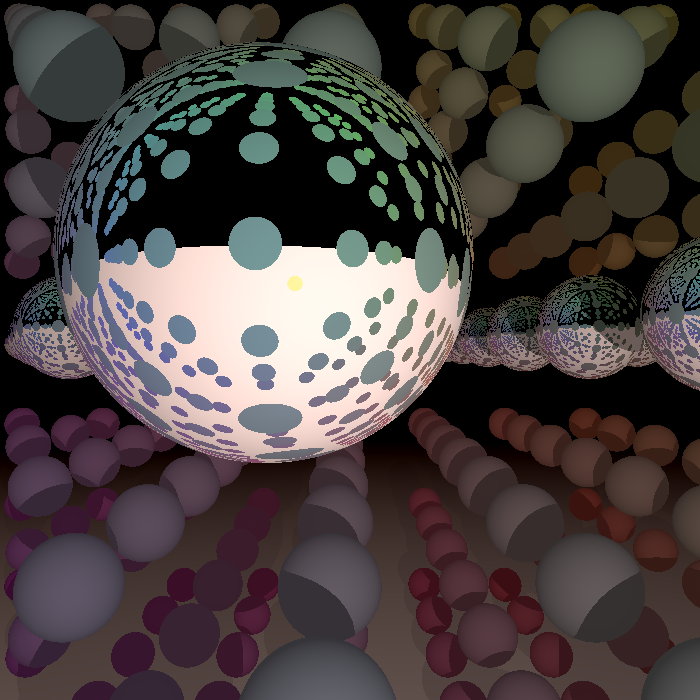
\includegraphics[width=90mm]{reflections.png}
\caption{Reflections that only take into account ambient lighting}
\label{fig:reflections}
\end{figure}

\subsection{Performance}
The raytracer is able to render a 700x700 pixel test scene with 1000 spheres and a moveable diffuse light source at speeds that make it interactive (see figure \ref{fig:testscene}). Using the CPU, this scene takes 1.28 seconds per frame (0.78 frames per second). Using the Radeon 7970, the scene takes 0.055 seconds per frame (18 frames per second). If the number of spheres is reduced to 216, the Radeon 7970 can render the scene at 60 frames per second.

\begin{figure}[ht!]
\centering
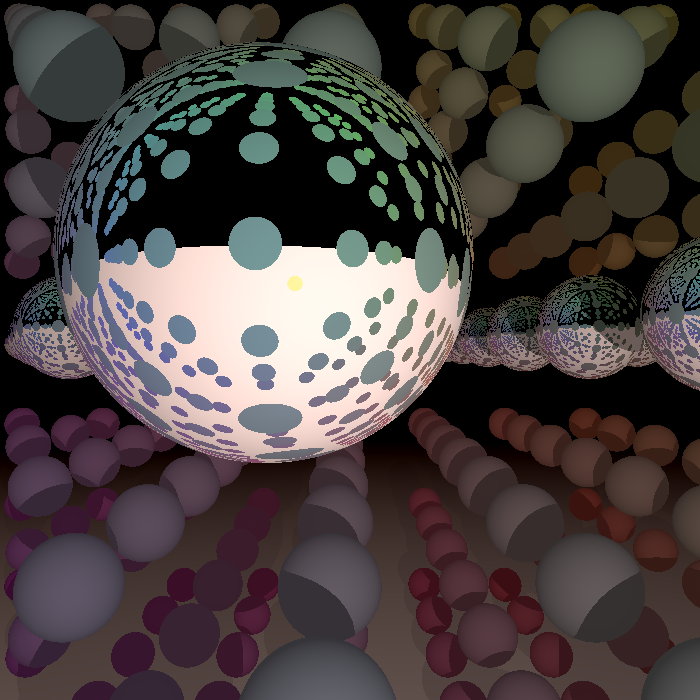
\includegraphics[width=90mm]{reflections.png}
\caption{Test scene with 1000 spheres and ground plane}
\label{fig:testscene}
\end{figure}

\section{Mankalah Minimax AI}


\section{Economics Simulation}


\section{\_\_local Memory malloc()}


\end{document}
